%%% LaTeX Template: Two column article
%%%
%%% Source: http://www.howtotex.com/
%%% Feel free to distribute this template, but please keep to referal to http://www.howtotex.com/ here.
%%% Date: February 2011

%%% Preamble
\documentclass[	DIV=calc,%
							paper=a4,%
							fontsize=12pt,%
							onecolumn]{scrartcl}	 					% KOMA-article class

\usepackage{lipsum}		
\usepackage{lscape}											% Package to create dummy text
\usepackage[brazil]{babel}										% English language/hyphenation
\usepackage[protrusion=true,expansion=true]{microtype}				% Better typography
\usepackage{amsmath,amsfonts,amsthm}					% Math packages
\usepackage[pdftex]{graphicx}									% Enable pdflatex
\usepackage[svgnames]{xcolor}									% Enabling colors by their 'svgnames'
\usepackage[hang, small,labelfont=bf,up,textfont=it,up]{caption}	% Custom captions under/above floats
\usepackage{epstopdf}												% Converts .eps to .pdf
\usepackage{subfig}													% Subfigures
\usepackage{booktabs}												% Nicer tables
\usepackage{fix-cm}													% Custom fontsizes
\usepackage[utf8]{inputenc}
\usepackage[top=2.5cm, bottom=2.5cm, left=2.5cm, right=2.5cm]{geometry}
\usepackage[ddmmyyyy]{datetime}
\addto\captionsenglish{%
	\renewcommand\tablename{Tabela}
	\renewcommand\figurename{Figura}
} 
 

 
%%% Custom sectioning (sectsty package)
\usepackage{sectsty}													% Custom sectioning (see below)
\allsectionsfont{%															% Change font of al section commands
	\usefont{OT1}{phv}{b}{n}%										% bch-b-n: CharterBT-Bold font
	}

\sectionfont{%																% Change font of \section command
	\usefont{OT1}{phv}{b}{n}%										% bch-b-n: CharterBT-Bold font
	}



%%% Headers and footers
\usepackage{fancyhdr}												% Needed to define custom headers/footers
	\pagestyle{fancy}														% Enabling the custom headers/footers
\usepackage{lastpage}	

% Header (empty)
\lhead{}
\chead{}
\rhead{}
% Footer (you may change this to your own needs)

%% ====================================
%% ====================================
%% mude o rodape  do projeto
%% ====================================
%% ====================================

\lfoot{\footnotesize \texttt{Cabeamento estruturado} \textbullet ~Modelo de projeto}


\cfoot{}
\rfoot{\footnotesize página \thepage\ de \pageref{LastPage}}	% "Page 1 of 2"
\renewcommand{\headrulewidth}{0.0pt}
\renewcommand{\footrulewidth}{0.4pt}



%%% Creating an initial of the very first character of the content
\usepackage{lettrine}
\newcommand{\initial}[1]{%
     \lettrine[lines=3,lhang=0.3,nindent=0em]{
     				\color{DarkGoldenrod}
     				{\textsf{#1}}}{}}



%%% Title, author and date metadata
\usepackage{titling}															% For custom titles

\newcommand{\HorRule}{\color{DarkGoldenrod}%			% Creating a horizontal rule
									  	\rule{\linewidth}{1pt}%
										}

\pretitle{\vspace{-30pt} \begin{flushleft} \HorRule 
				\fontsize{50}{50} \usefont{OT1}{phv}{b}{n} \color{DarkRed} \selectfont 
				}

%% ====================================
%% ====================================
%% mude o titulo  do projeto
%% ====================================
%% ====================================

\title{Projeto de Cabeamento Estruturado Comercial}					% Title of your article goes here

%% ====================================



\posttitle{\par\end{flushleft}\vskip 0.5em}

\preauthor{\begin{flushleft}
					\large \lineskip 0.5em \usefont{OT1}{phv}{b}{sl} \color{DarkRed}}
\author{Marcos Felipe da Silva }  	% Author name goes here


\postauthor{\footnotesize \usefont{OT1}{phv}{m}{sl} \color{Black} 
					\\Universidade Tecnológica Federal do Paraná - Câmpus Cornélio Procópio 								% Institution of author
					\par\end{flushleft}\HorRule}

\date{}																				% No date




%%% Begin document
\begin{document}
\maketitle
\thispagestyle{fancy} 	
\thispagestyle{empty}		% Enabling the custom headers/footers for the first page 
% The first character should be within \initial{}




%% ====================================
%% ====================================
%% mude o resumo  do projeto
%% ====================================
%% ====================================

\initial{E}\textbf{ste projeto fictício tem como objetivo apresentar soluções para a substituição de uma estrutura de cabeamento de um estabelecimento comercial real. A estrutura abrange uma área de aproximadamente 200 m$^{2}$. O plano de certificação da rede está basicamente no âmbito da norma EIA/TIA 568.  A planta da fundação será apresentada no escopo deste projeto, para melhor representação da área de abrangência da estrutura cabeada. Por fim, será apresentado o orçamento final do projeto, bem como, o plano de manutenção e riscos.}


%% ====================================
\begin{figure}
	\centering
	
\includegraphics{utfpr}
\end{figure}

\vspace{2cm}
\centerline{\textit{\textbf{\today}}}

\clearpage
    \renewcommand*\listfigurename{Lista de figuras}
\listoffigures

\renewcommand*\listtablename{Lista de tabelas}
\listoftables




\clearpage
\renewcommand{\contentsname}{Sumário}
\tableofcontents
\clearpage

%% ====================================
%% ====================================
%% Inicio do texto
%% ====================================
%% ====================================
\section{Introdução}

Este é um projeto fictício, que tem como objetivo apresentar uma solução de cabeamento estruturado para uma empresa real. A empresa em estudo é um comércio de crachás e equipamentos de ponto eletrônico. Nesta empresa existem 10 colaboradores, eles são: técnicos de hardware, secretários, técnicos de suporte de software, desenvolvedores de software e atendentes. Nas etapas subsequentes serão apresentadas as informações a respeito dos equipamentos presentes na organização e as características da empresa.

\subsection{Benefícios}

A nova estrutura proporcionará uma maior facilidade de gerenciamento do sistema de cabeamento estruturado. A organização da estrutura facilita a manutenção e operação dos técnicos, diminuindo a carga de trabalho humana e contribuindo para melhor entendimento de um sistema descomplicado.
Também reduzirá os custos, uma estrutura mais organizada não dependerá de tantos profissionais especializados para operar e realizar manutenções no sistema. A manutenção da estrutura se torna menos frequente.
 
A nova estrutura torna a capacidade de expansão muito maior, para movimentação, adição ou alteração de recursos na estrutura. Com tempo isso se transforma em maior retorno financeiro, ou menor perda se comparada a estrutura antiga, para empresa. Com essa capacidade de expansão, a estrutura promove o aumento de largura de banda, ou seja, suportará com folga as aplicações que demanda fluxo maior de dados como: multimídia e videoconferências.

Outro ponto de vantagem é a estética promovida com a nova estrutura. Quando se tem uma organização de cabos e aparatos por eletrocalhas, a empresa se beneficia com uma estrutura mais adequada, operacional e visualmente mais agradável se comparada as estruturas atuais e seu emaranhado de fios. Isso tem impactato inclusive na imagem externa da empresa como marca.

\subsection{Organizações Envolvidas}
No projeto haverá apenas uma empresa envolvida, a empresa Crachá Digital. Portanto, o projeto se trata de uma estrutura independente, que não delega recurso para outra empresa, e nem sequer é um subsistema de outra rede.



\section{Estado atual}
As características da rede atual, seus passivos e uma breve avaliação por parte dos usuários da rede.

\begin{itemize}
	\item Os passivos da rede: a estrutura conta com uma mini Rack de parede acoplada na sala de servidores (Figura 1). Há cabos de rede no forro das instalações interligando os equipamentos e o switch. Também há pequenas calhas de plástico para acabamento dos cabos de UTP nas paredes;
	
	\item As principais reclamações dos usuários: falta de suporte a tecnologias que demandam maior fluxo de dados, como videoconferências e acesso a desktop remoto. Isso se deve pelo fato da rede atual ser apenas Mbit.
	
	\item Observações: Há seções na rede que requerem cobertura completa de cabos, pois a construção conta com salas externas que não tem cobertura entre a seção principal e algumas seções periféricas. A não cobertura dos cabos faz com que o cabo sofra erosão por chuva e deterioração por insolação;
	
\end{itemize}

\section{Requisitos}
Crie uma enumeração dos requisitos do projeto.

\section{Usuários e Aplicativos}
A seguir será apresentada uma relação de possíveis usuários, seu número estimado e aplicativos executados em alguns equipamentos na infraestrutura. 
 

\subsection{Usuários}
Tipos de equipamento:
\begin{itemize}
	\item Terminais de trabalho (computadores). Entre 10 e 50 terminais;
	\item Telefones PABX. Entre 5 e 15 terminais;
	\item Câmeras de segurança (interna e externa). Entre 2 e 10 câmeras;
	\item Terminais de registros de ponto eletrônico. Entre 1 e 4 terminais;
	\item Dispositivos de impressão (impressoras). Entre 1 e 5 dispositivos;
	\item Smartv. Entre 1 e 3 equipamentos;
\end{itemize}


\subsection{Aplicativos}

Relação de aplicativos críticos utilizados nos equipamentos:

\begin{itemize}
	\item Serviço de VoIP;
	\item Aplicações de video chamadas (exemplo: Skype);
	\item Aplicações de acesso remoto (exemplo: Anydesk);
	\item Aplicações com alta demanda de conexões por socket (exemplo: Helpdesk);
	\item Alto fluxo de requisições para impressão em equipamentos de impressão;
\end{itemize}



\section{Estrutura predial existente}

A planta (Figura \ref{planta-atual}) representa a construção atual. A construção conta conta com apenas um andar. A extensão máxima de área construída útil é de aproximadamente 44 metros. Com uma largura medindo cerca de 12 metros. A sala do servidor, onde é centralizada a rede, fica no centro da construção, isso facilita a distribuição de cabos no entorno do edifício.

Há também uma área externa, desprendida da construção principal, a sala de manutenção. Esta área requer cuidado especial, pois a passagem de cabeamento deve ser protegida do ambiente externo.

\begin{figure}[h]
	\centering
	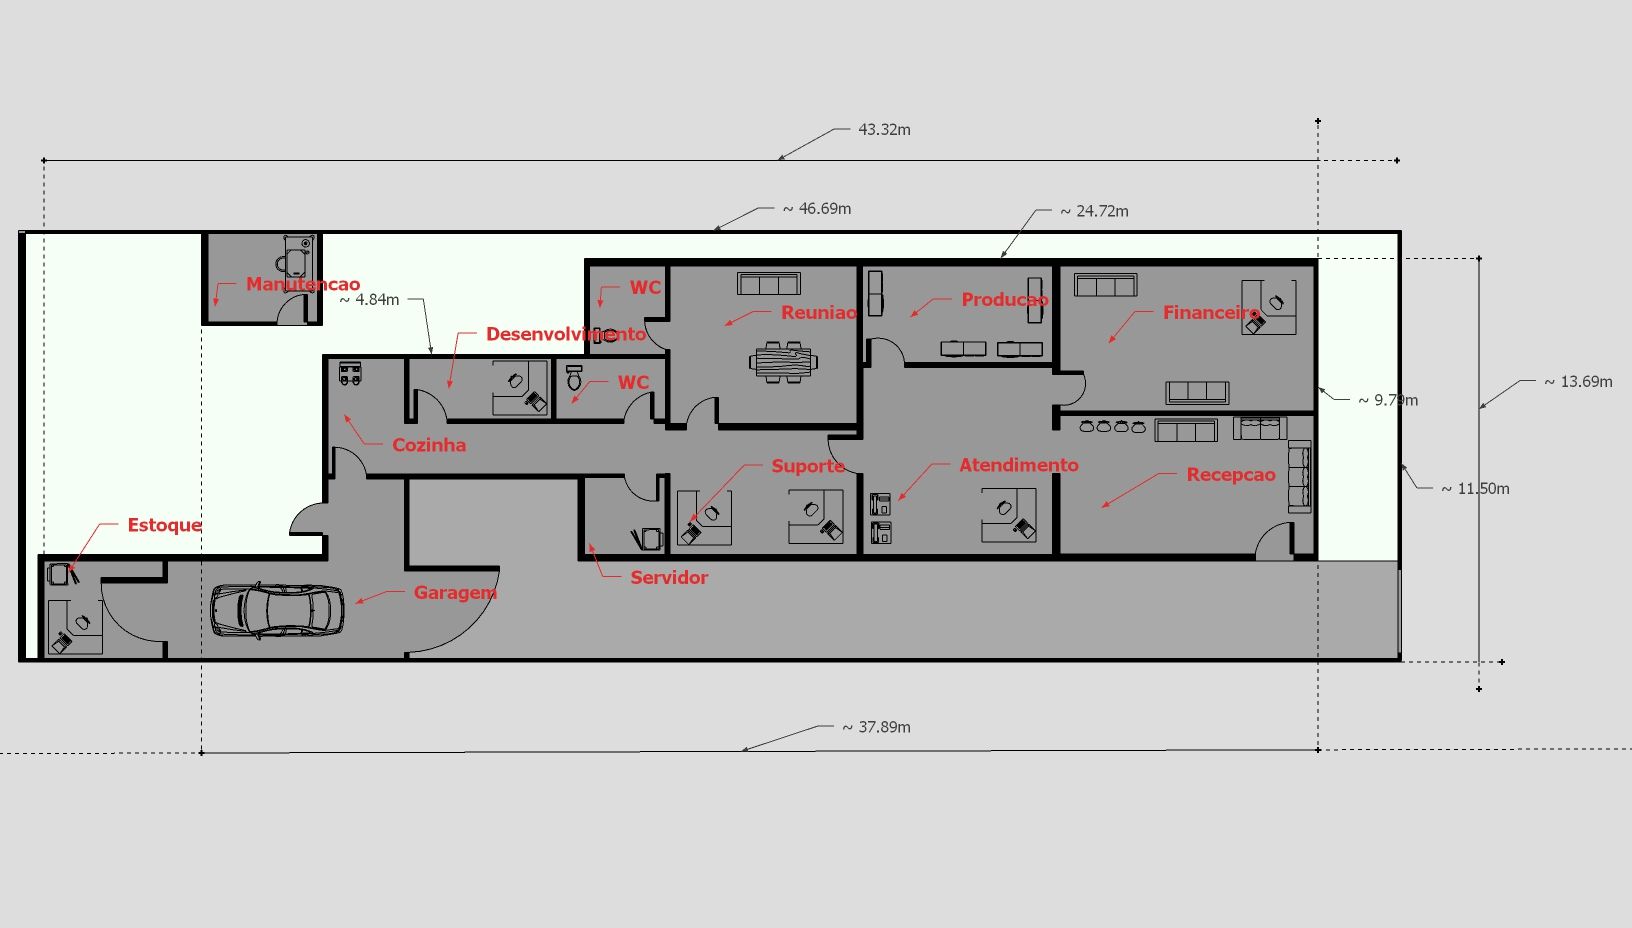
\includegraphics[width=\textwidth]{planta-atual}
	\caption{Planta Atual}
	\label{planta-atual}
\end{figure}

\section{Planta Lógica - Elementos estruturados}

\subsection{Estado atual}


\subsection{Topologia}
Proposta futura, proposta após implantação.
Deve conter o diagrama da rede. Atente-se a redundância  e ligações truncadas.
Deve explicar todos termos e componentes utilizados nestas plantas. Por exemplo: entrance facility, work area, horizontal cabling, etc..

Todos os elementos das figuras devem ser explicados. 
Crie esboço da configuração dos racks e brackets. Explique cada um dos componentes. Você pode criar uma tabela contendo figuras dentro, ou criar uma tabela e incluí-la como imagem. Por exemplo, verifique a tabela \ref{tab1}.

\begin{table}[h!]
\centering
\caption{Exemplo de tabela explicativa}
\label{tab1}
\begin{tabular}{|l|l|l|}
\hline
\multicolumn{3}{|l|}{Figura na Tabela} \\ \hline
1        & Rack          & \includegraphics[scale=0.2]{fig1}        \\ \hline
2        & Rack 2        & \includegraphics[scale=0.2]{fig1}        \\ \hline
\end{tabular}
\end{table}

\subsection{Encaminhamento}
Eletrodutos, calhas, e qualquer material em que os cabos serão alojados/alocados.

\subsection{Memorial descritivo}

Relacione todos os equipamentos passivos que serão utilizados, tipo, fabricante, quantidade.

\subsection{Identificação dos cabos}
Explique como os cabos serão identificados em seu projeto. Coloque uma relação dos cabos instalados e identificados.

\section{Implantação}
Estabeleça um cronograma de implantação:
Remoção de equipamentos existentes (destino para descarte), instalação dos condutores, instalação dos cabos, 
identificação dos cabos, montagem dos racks, certificação, etc... Crie atividades e estabeleça o tempo de execução. Se for um projeto real, indique também quais os responsáveis pela execução do projeto e de cada uma das etapas.

Defina marcas (e padrões) e fornecedores se for o caso. Atenção a contratados e subcontratados para a realização das atividades. Estabeleça a responsabilidade de execução da atividade e também da validação dela.

Utilize algum software para gerear o cronograma. Excel,etc. O fundamental é dividir em etapas, descrever e estimar o tempo de cada uma delas.

Segue uma relação de ferramentas:
http://asana.com/, 
https://trello.com/, 
http://www.ganttproject.biz/, 
http://www.orangescrum.org/. 

\section{Plano de certificação}
Quais seriam as etapas para a certificação? 
Quais os locais e horários para execução da certificação na rede? Toda rede será certificada?
Como os testes seriam executados?
Quais relatórios de certificação serão (ou deveriam ser) entregues? 

\section{Plano de manutenção}

Revisões periódicas na rede, emissão de certificados para novos pontos.

\subsection{Plano de expansão}
Existe um plano de expansão? Quantos novos pontos poderão ser acrecidos na rede, antes de migração de equipamentos na camada 2? Se houver expansão, quais equipamentos deverão ser direcionados para as estremidades da rede? 

\section{Risco}
Enumerar e explicar os riscos do projeto.

\section{Orçamento}
Crie uma relação de orçamentos baseado na seções anteriores.

\section{Recomendações}
Observações e recomendações para o cliente.

\section{Referências bibliográficas}
Utilize o mendley, o jabref ou diretamente o bibtex para gerenciar suas referências biliográficas. As referências são criadas automaticamente de acordo com o uso no texto.

Exemplo: Redes de computadores, segundo \cite{t2013} é considerada..... Já \cite{kurose2010} apresenta uma versão...

Analisando os pressupostos de \cite{ref3} e \cite{ref4} concluimos que....


\renewcommand\refname{} %%Referências bibliográficas}  
\bibliographystyle{ieeetr}
\bibliography{referencias}  

%% ***********************************************************************
%% === remover daqui =====================================================
%% ***********************************************************************
=================================================
\section{Elementos textuais - Alguns exemplos}

Esta seção apresenta exemplos de elementos textuais. \textbf{Remova-a da versão final do texto}.


\subsection{Colocar elementos em itens}

Texto antes da lista

\begin{itemize}
	\item First item in a list 
	\item Second item in a list 
	\item Third item in a list
\end{itemize}

\subsubsection{Uma subseção de terceiro nivel}

Exemplo de uma subseção

\subsection{Tabelas}

Utilize o site http://www.tablesgenerator.com/ para elaborar as tabelas de seu trabalho.
Para adicionar uma tabela utilize: a tag input, passando o arquivo da tabela como parametro

\begin{table}[h!] % coloque h! para forcar a posicao
\centering
\caption{Modifique a legenda e crie um label}
\label{tab2} %com este label vc faz referencia no texto
\begin{tabular}{|l|l|l|l|l|}
\hline
\multicolumn{1}{|c|}{\textbf{Este é um exemplo de tabela}} & \multicolumn{2}{c|}{\textbf{C1}} & \multicolumn{2}{c|}{\textbf{C2}} \\ \hline
Você pode criar a tabela no excel                          & 1              & 2               & 3               & 4              \\ \hline
Exportar para CSV                                          & 5              & 6               & 7               & 8              \\ \hline
E importar no Table Generator                              & 9              & 10              &                 &                \\ \hline
\multicolumn{5}{|c|}{\textit{Gere o tex, e adicione em seu arquivo}}                                                             \\ \hline
\end{tabular}
\end{table}

Dentro do arquivo você deve definir o label e pode utilizá-lo para referenciar. Exemplo:
Na tab \ref{tab2} temos a relação de ....


Você também pode modificar a tabela manualmente, incluindo, por exemplo h! dentro de sua definição. Veja no exemplo tab2.tex

\subsection{Figuras}



\begin{figure}
\centering
\includegraphics[width=\textwidth]{fig1}
\caption{Exemplo de figura com escala horizontal}
\label{fig1}
\end{figure}


\begin{figure}
	\centering
	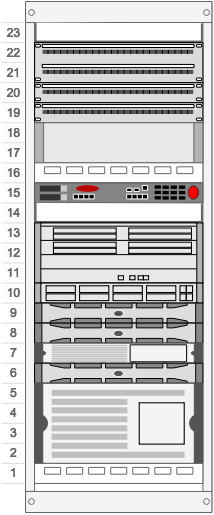
\includegraphics[]{fig2}
	\caption{Exemplo de figura sem escala}
	\label{fig2}
\end{figure}

Você pode rotacionar figuras também. Para isso utilize o parâmetro angle=-90. Repare que a escala da figura foi modificada pelo parametro height. Você também pode utilizar scale

\begin{figure}
	\centering
	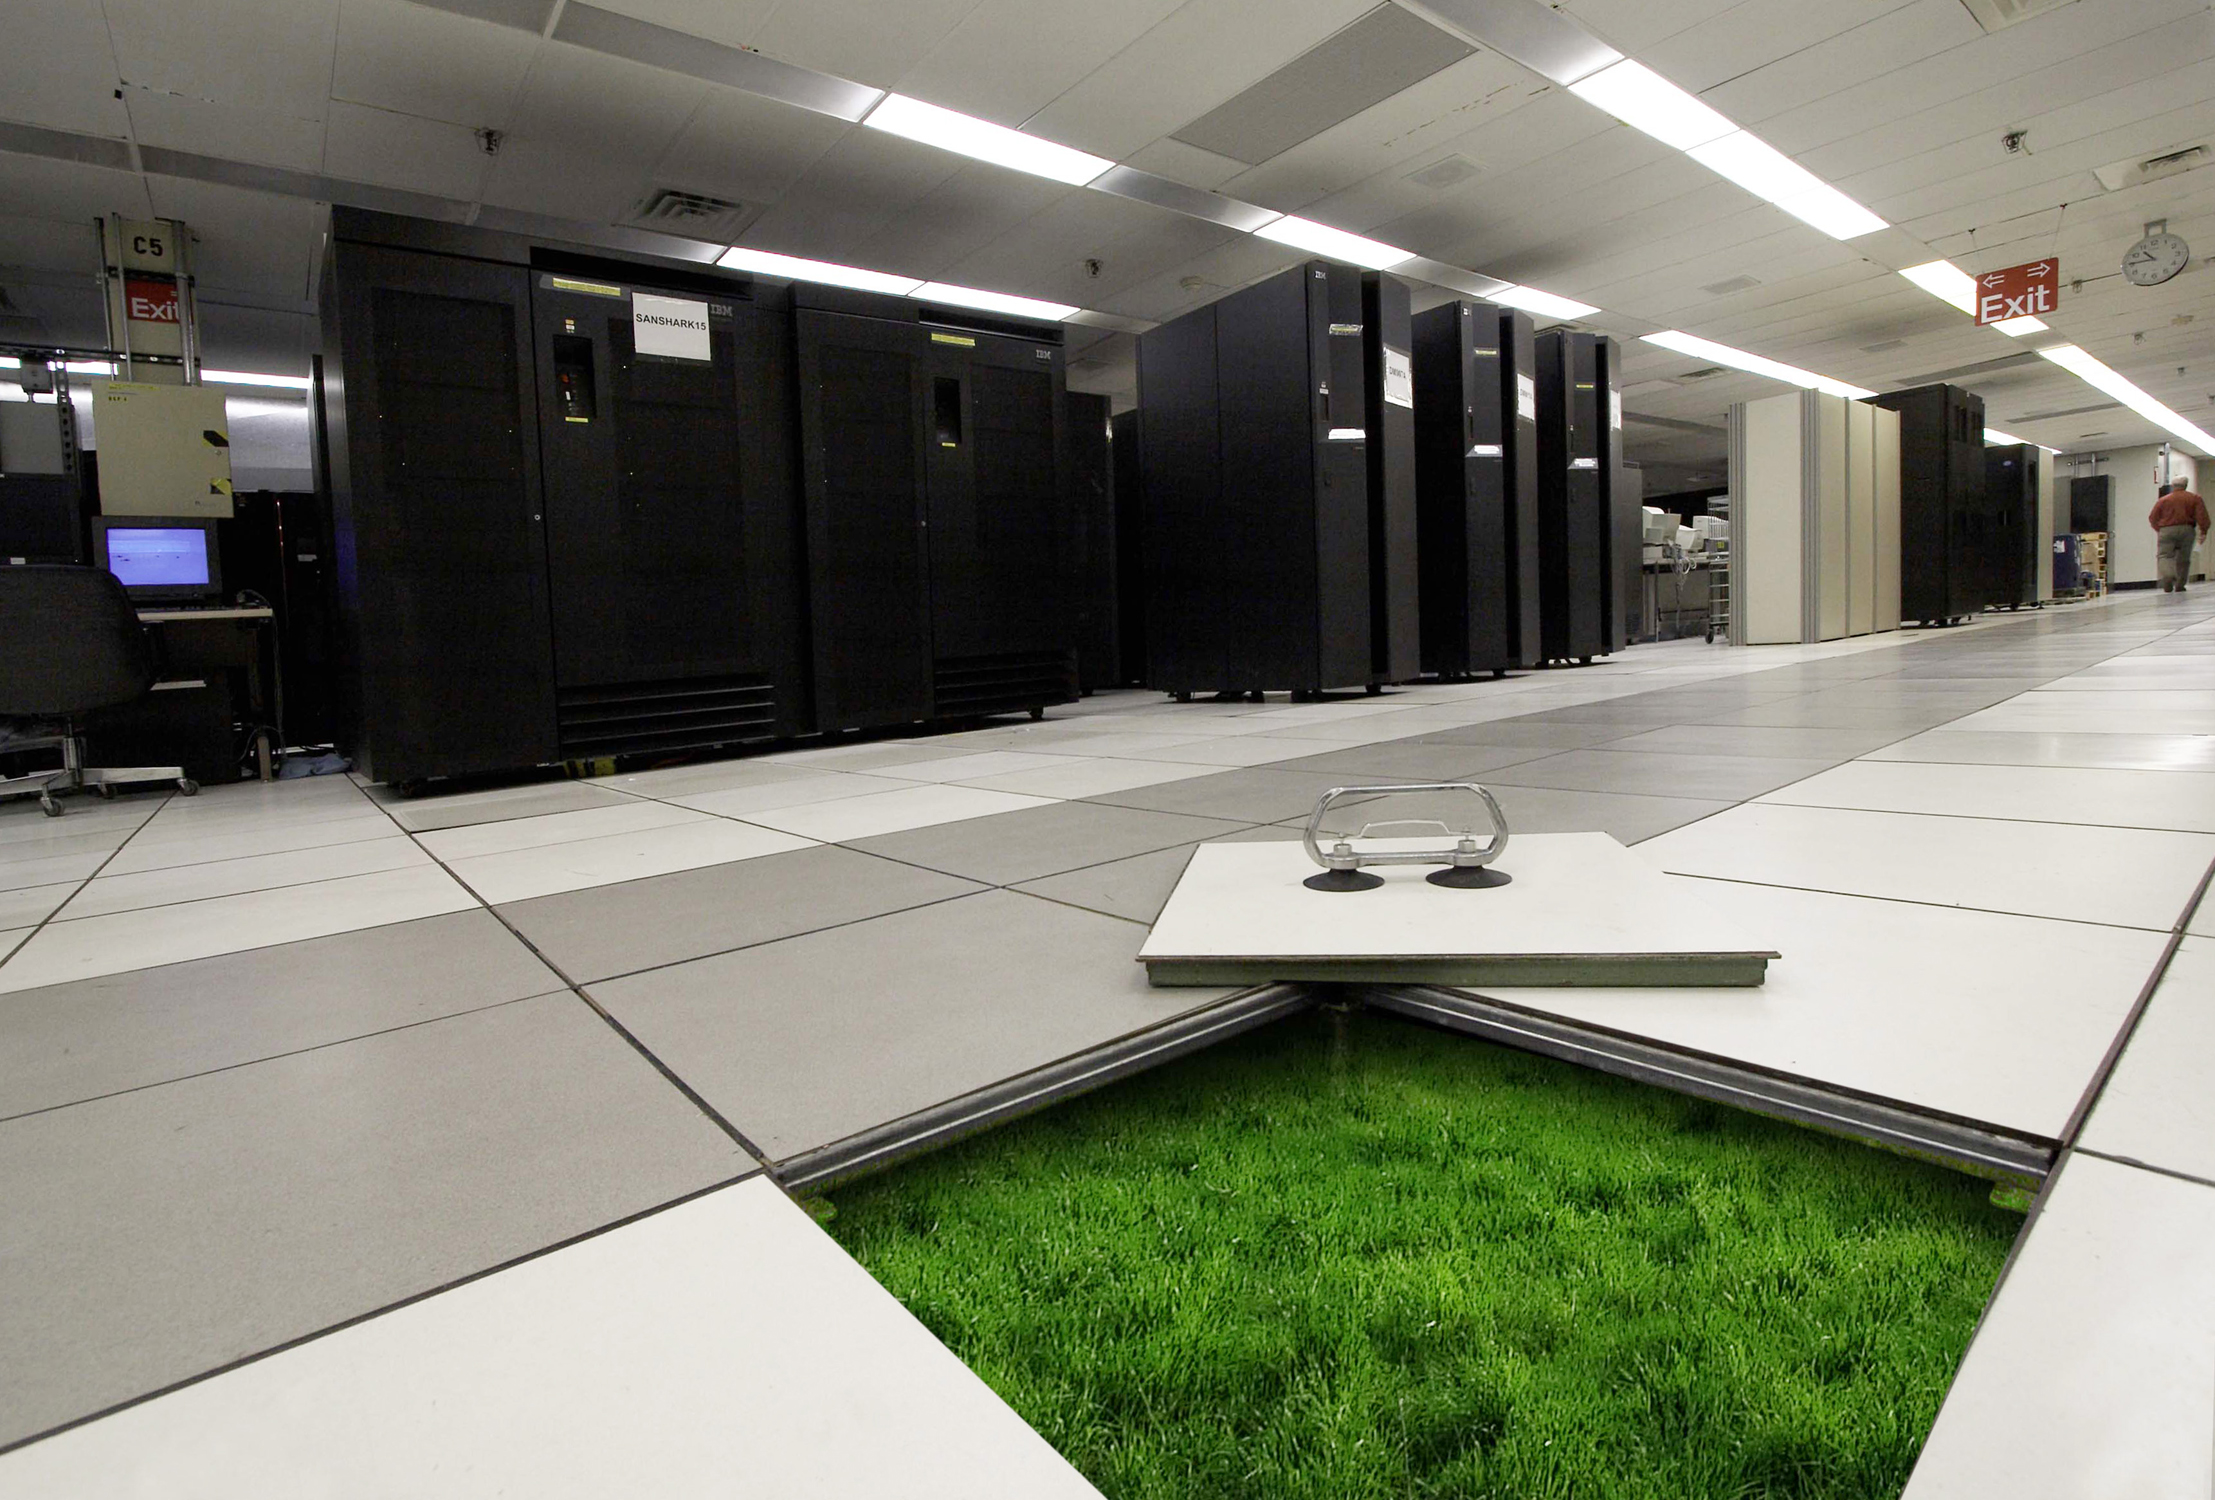
\includegraphics[height=\textwidth,angle=-90]{fig3}
	\caption{Exemplo de figura rotacionada}
	\label{fig3}
\end{figure}

\subsubsection{Resumo gráfico}

Você pode optar por fazer um resumo no formato de mapa mental/conceitual. 
Aqui foi utilizado o site https://app.mindmup.com para gerar o mapa.

Para utilizar o resumo gráfico, remova o texto da seção resumo (linha 137) e inclua o código para inserir a figura, conforme figura \ref{fig4}

\begin{figure}[h]
	\centering
	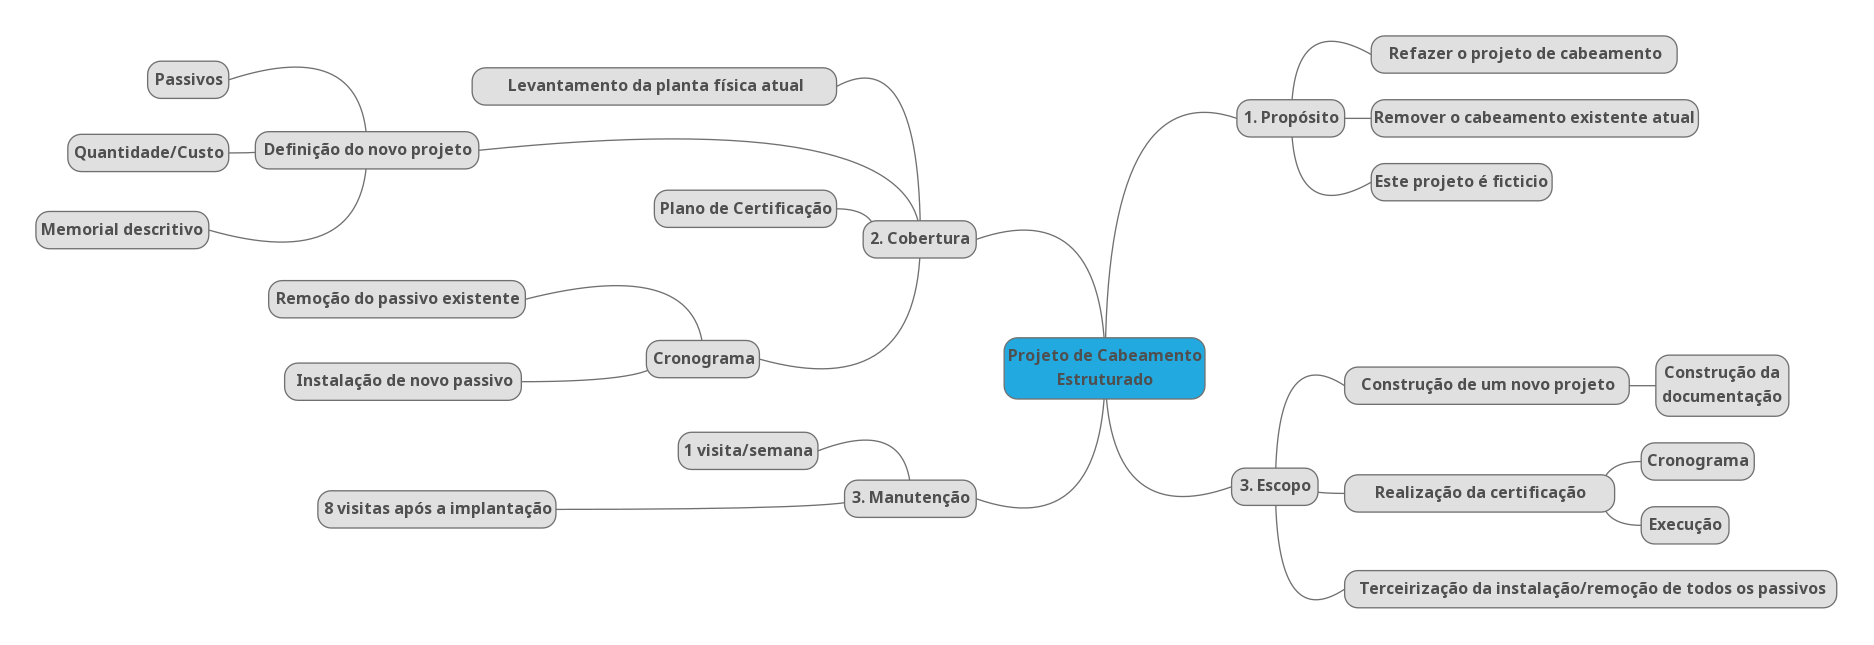
\includegraphics[width=\textwidth,height=5cm,keepaspectratio]{fig4}
	\caption{Exemplo de resumo gráfico}
	\label{fig4}	
\end{figure}

%% ***********************************************************************
%% === ate aqui    =====  ================================================
%% ***********************************************************************

\end{document}